\chapter{Travail effectués}
Dans ce chapitre je décrie les tâches accomplies lors de ce stage, ainsi que les difficultés rencontrées.
\section{Modification du plugin Gstreamer MPEG-TS}
% Pourquoi
Comme expliqué précédemment, mon stage s’inscrit dans une continuité, et donc a pour but d'améliorer le système déjà présent. Avant ma participation au projet, le système prenait des flux vidéo de sources différentes (caméras de sécurité, fichier vidéo, etc.), pour ensuite faire passer ce flux vidéo par des briques algorithmiques de traitement d'images (détection des visages, détection de mouvement...). De ce traitement d'images on extrait des métadonnées, dans le cas de la détection de visages nous obtenons des rectangles représentant la surface recouvrants les visages. Ces métadonnées étaient formatées au format ONVIF\footnote{ONVIF où "Open Network video interface Forum" est une convention internationale, qui a pour but de faciliter le développement du standard pour l'interfaçage des produits de sécurité avec adresse IP, exemple caméra de sécurité}. Le flux vidéo et le flux de métadonnées sont "timestamper", afin qu'ils soient synchronisés plus tard, puis ils sont ajoutés au conteneur MKV\footnote{le format MKV (Matroska Video) est un format vidéo entièrement libre. Plus exactement il s'agit d'un conteneur (d'où le nom Matroska, en référence aux poupées russes) permettant de contenir de la vidéo (Divx, Xvid, RV9, etc.), du son (MP3, Ogg, MP2, AC3, DTS, AAC, PCM), ainsi que des sous-titres (SRT, ASS, SSA, USF, etc.) dans un même fichier.} pour la transmission. Ainsi, le flux de métadonnées était passé en sous-titres dans le dans MKV. Or, le format MKV recevait les métadonnées formatées au format ONVIF (sous forme XML), il reformatait de nouveau ce flux, ce qui corrompait les métadonnées. C'est de cette problématique que découle mon stage, on avait besoin de transmettre le flux vidéo/métadonnées au travers d'un protocole standard sans avoir modifié le format des métadonnées. Ainsi nous nous sommes intéresser au protocole MPEG-TS.
% qu'est c'est

\subsection{Architecture de MPEG-TS}
MPEG-TS ou MPEG Transport Stream permet de contenir du flux digital (audio, vidéo, ou bien privé tel que des sous-titres). Il intègre aussi la synchronisation de flux et la correction  d'erreur lors d'une perte de paquet. L'autre intérêt de MPEG-TS est qu'il peut contenir plusieurs "programmes" dans un flux. Chaque programme peut contenir N flux vidéo ou audio ou privés. Chacun de ces flux à un identifiant ou "PID"\footnote{Packet ID} et chaque programme a un PID\footnote{dans ce cas si PID veut dire Program ID}. Les programmes sont enregistrés dans une PMT\footnote{Programme Map table} une table des programmes regroupant les différents programmes. Les PMT sont ensuite enregistrés dans une PAT\footnote{Programme Association table}.

\begin{figure}[!h]
  \centering
  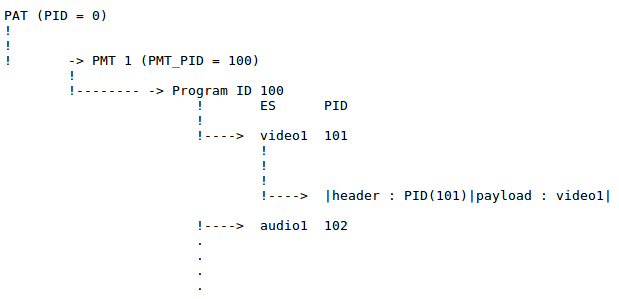
\includegraphics[scale=0.7]{figures/ts_diag}
  \caption{schéma de l'encapsulation de média dans MPEG-TS}
\end{figure}

\begin{figure}[!h]
  \centering
  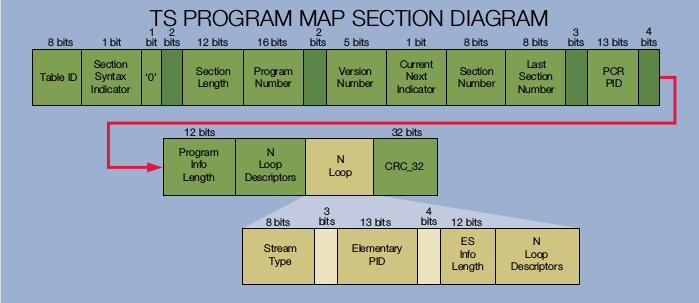
\includegraphics[scale=0.6]{figures/ts}
  \caption{schéma d'une trame d'une section Transport Stream}
\end{figure}

\subsection{Explication des plugins mpegtsmux et tsdemux}
% qu'est ce que j'ai fait ?
Suite à l'étude de MPEG-TS au niveau architecturale, je me suis m'y à lecture du code de son implémentation sous Gstreamer. Le l'implémentation se compose en deux partie,
la partie "multiplexage",et la partie "démultiplexage". Comme presque tout les plugins, elle sont codés en C avec la librairie GObject\footnote{GObject est une interface de programmation et une bibliothèque logicielle multiplate-forme publiée sous licence libre (LGPL), qui permet de manipuler des objets, ainsi que d'avoir accès à une palette d'objets élémentaires. Deplus, GObject s'interface très bien avec d'autres langages de programmation comme Python ou bien Vala.}.\\
  \paragraph{Le plugin mpegtsmux}
Le multiplexage se fait au travers du plugin \textbf{mpegtsmux}. Le flux de données entre depuis le pad d'entrée\footnote{cf. \ref{principe gst}} avec une négociation des caps qui donne le type multimédia du flux (exemple : vidéo/x-raw, qui est un flux vidéo pur sans encodage) puis le flux est découpé en paquet "timestamper", et identifier. Ainsi sont traités tous les flux. Ensuite tous les paquets sont "entrelacés" dans un seul flux puis mis à disposition sur le pad de sortie.
  \paragraph{Le plugin mpegtsdemux}
Le démultiplexage fonctionne à l'inverse. Les paquets reçus sont analysé par \textbf{tsparse}, plugin qui parse les paquets TS et qui les donne à \textbf{mpegtsdemux} . Ensuite le mpegtsdemux refabrique les différents flux et crée un pad à la demande (ou "request pad" dans la littérature anglophone) par flux. Il suffit donc de se connecter à ces pads de sortie pour avoir le flux que l'on souhaite

\subsection{Modifications apportés au plugins}

\paragraph{Ajout d'un nouveau types élémentaire:} Les plugins permettent de muxer et demuxer du flux multimédia connue, dont le type multimédia à un code\footnote{cf. \url{https://en.wikipedia.org/wiki/Program-specific_information#Elementary_stream_types}}. Or pour des raisons d'interopérabilité avec d'autres plateformes et logiciels nous avons décidé de créer un nouveau type élémentaire dans le code. Ce type est ajouté aux deux plugins \footnote{cf. \ref{tsmux_annexes_h}}.
\paragraph{Modifications du muxer pour accepter le nouveau type:} Après avoir ajouté un nouveau type élémentaire, il faut que lorsque le muxage soit fait, on puisse identifier le flux avec son type et lui donner son ID . Cela est fait en modifiant la méthode \textbf{mpegtsmux\_create\_stream}. Lors de la négociation des caps on récupère le type du flux, ici "application/x-private". Ensuite on test le type et on attribut le l'"element steam type" pour le flux, dans notre cas \textbf{TSMUX\_ST\_PS\_KLV}. Ensuite on attribut le PID du flux, grâce à la méthode de \textbf{tsmux\_create\_stream}, soit en passant un entier de 32 bit, soit la méthode
boucle jusqu'a trouvé un PID vacant.
\paragraph{modifications du demuxer:}  Les modifications du démuxer sont plus simples puisqu'il s'agit récupérer un flux de type "application/x-private" puis d'ouvrir un pad de sortie et de fournir le flux demandé . Pour ce faire j'ai ajouté un test dans la méthode "create\_pad\_for\_stream" puis j'ai créé les caps qui convenaient.
\begin{lstlisting}[language=C, caption=création de caps pour le flux sortant,label=demux_c]
...
case DRF_ID_XPRIVATE:
          sparse = TRUE;
          is_private = TRUE;
          caps = gst_caps_new_simple ("application/x-private",
              "parsed", G_TYPE_BOOLEAN, TRUE, NULL);
          break;
...
\end{lstlisting}

Après test j'ai pu transmettre du flux vidéo accompagné de données générer aléatoirement et donc pue passer à la deuxième partie de mon stage .

\section{Projet SisellBox}

Pour la seconde phase de mon stage, il m'a été attribué de modifier et d'automatiser le système de provisionnement du système tournant sur VM. et ensuite de tester les plugins MPEG-TS dans le contexte de projet.

% Pourquoi j'ai Modification + - Sisell elements\\ - sboxstreamer\\
 \subsection{Étude de l'existant}
J'ai dans un premier temps étudié le projet dans son ensemble, voici une description non exhaustive du projet
  \begin{description}
   \item [ansible : ] contient tout ce qui concerne le provisionnement de la machine VM ainsi que la gestion des VMs avec Vagrant.
  \item [dataset : ] contient des vidéos de tests .
  \item [httpproxy : ] contient les configurations du serveur web nginx.
\item [sboxweb : ] contient l'interface web du projet, à cela ajouté le backend codé en Python Flaskr.
\item [simple\_stream : ] contient l'application de test que j'ai développée.
\item [sisell\_éléments : ] contient les briques algorithmiques de traitement d'images et interfacé avec Gstreamer sous forme de plugins
  \end{description}

 \subsection{mise à jour du système de provisionnement}
 % a quoi ressemblait l'archi avant puis ce que l'on en fait apres
La nouvelle architecture qui m'a été demandé d'implémenter à pour but de simplifier la compréhension du système de provisionnement mais aussi de simplifier les modifications futures. La découpe est la suivante :
  \begin{description}
   \item [1\_devenv] une brique réservée au provisionnement des outils qui mette en place un environnement de développement
   \item [2 \_streamers] partie installe les outils de développement nécessaires au streamer, principalement les paquets Gstreamer
   \item [3 \_streamers\_dev] rôles qui cherche les sources Gstreamer, les configure, les compile, et enfin fabrique des paquets Debian pour faciliter la gestion de ces paquets
   \item [4\_control] script qui compile et installe toutes sources et librairies qui sont responsables du contrôle au sens le plus abstrait de l'application. On peut y trouver les librairies grpc et Protobuf, ainsi que leurs binders Python.
   \item [5\_algo] brique consacré à l'installation des librairies Open Cv.
  \end{description}

  \begin{lstlisting}[caption=exemple de rôles Ansible ,label=ansible_exemple]
    - name: Install Mysql package
  yum: name={{ item }} state=present
  with_items:
   - mysql-server
   - MySQL-python

- name: Configure SELinux to start mysql on any port
  seboolean: name=mysql_connect_any state=true persistent=yes
  when: sestatus.rc != 0

- name: Create Mysql configuration file
  template: src=my.cnf.j2 dest=/etc/my.cnf
  notify:
  - restart mysql

- name: Start Mysql Service
  service: name=mysqld state=started enabled=yes

- name: Create Application Database
  mysql_db: name={{ dbname }} state=present

- name: Create Application DB User
  mysql_user: name={{ dbuser }} password={{ upassword }}
  \end{lstlisting}


 Ensuite, pour créer une machine virtuelle à l'aide Vagrant et la provisionner, il suffit de taper la commande :
  \begin{lstlisting}[language=bash]
  vagrant up --provision
  \end{lstlisting}
 Une VM est lancé on peut donc y accéder depuis un lien ssh sécurisé que Vagrant fournit :
  \begin{lstlisting}[language=bash]
  vagrant ssh
  \end{lstlisting}


 \subsection{Application de Test}
La finalité de mon stage fut de pouvoir streamer un flux MPEG-TS contenant un flux vidéo, et des métadonnées obtenues depuis des algorithmiques de traitement d'images, au travers du protocole RTP. Ainsi mon but a été de transmettre depuis une VM jusqu'à ma machine.
Voici les pipelines réalisés :

\paragraph{Coté streamer: }

\begin{verbatim}
 GST_DEBUG=3 GST_DEBUG_DUMP_DOT_DIR=./stream \
	 gst-launch-1.0 filesrc location=/dataset/videoMP4.mp4 do-timestamp=true !\
	   decodebin ! video/x-raw,format=I420 ! tee name=src  \
	 mpegtsmux name=m ! video/mpegts ! rtpmp2tpay ! udpsink host=10.1.75.173 port=5555 \
	 src. ! queue name=post_face_queue max-size-time=0 max-size-bytes=0\
	   max-size-buffers=0  ! videoconvert ! video/x-raw,format=BGR ! \
	     owfacedetect name=face !\
	       capssetter caps="application/x-private,parsed=true"\
		 replace=true join=false ! m. \
	 src. ! queue name=video_q  ! x264enc ! m.
\end{verbatim}
Le pipeline ci-dessus est celui qui se charge de streamer. On peut lire les variables GST\_DEBUG et GST\_DEBUG\_DUMP\_DOT\_DIR qui sont utiles pour avoir des logs plus verbeux et indiqués où l'on veut que les graphes .dot soit générer. Le plugin \textbf{filesrc} cherche le fichier MP4, le lit, et le fournit sur son pad de sortie. La propriété "do timestamp" est mise à true afin que le plugin écrive des paquets timestamper. le flux vidéo et ensuite donné à un élément appelé \textbf{decodebin}. Il va se charger de décoder le flux et retourner sur son pad se sortit le type demandé en caps, ici "vidéo/x-raw, format=I420". la vidéo décodée va être récupérée par l'élément \textbf{tee} que l'on nomme "src". Il se charge de dupliquer sur le flux pour autant de branche qui demande. La prémière branche fourni est celle-ci reliée au plugin mpegtsmux patché, tandis que la deuxième branche convertie l'encodage des couleurs du flux vidéo d'I420 vers du BGR\footnote{BGR: Blue, Green, Red} pour le plugin de détection owfacedetect. Les métadonnées sont ensuite données, post-négociation de caps, au multiplexeur. Il en va de même pour la vidéo qui est encodée en H.264 par \textbf{x264enc}. Les muxer produits des paquets TS qu'il fournit au plugin \textbf{rtpmp2tpay} qui les empaquette dans des paquets RTP pour ensuite les envoyer par UDP grâce au plugin \textbf{udpsink} .


\paragraph{Coté recoder: }

\begin{verbatim}
  GST_DEBUG=4 GST_DEBUG_DUMP_DOT_DIR=./record \
	 gst-launch-1.0 udpsrc port=5555 ! application/x-rtp,media=video,clock-rate=90000,\
	   encoding-name=MP2T ! rtpmp2tdepay ! tsparse ! tsdemux name=d \
	 d.private_0041 ! queue name=meta_queue ! filesink location=lol\
	 d.video_0042 !  queue name=video_queue ! video/x-h264 ! h264parse ! \
	   avimux ! filesink location=lol.avi  \
\end{verbatim}
ce pipeline fait l'inverse du pipeline streamer . On récupère le flux RTP/TS au travers d'UDP, puis \textbf{rtpmp2tdepay} dés-empaquette les paquets TS. Ces derniers sont analysés par \textbf{tsparse} qui fournit au plugin \textbf{tsdemux} un flux TS à demuxer. Ensuite il suffit de lire les bons pads pour avoir ce que l'on veut. Comme par exemple ci-dessus le flux privé est sur le pad "private\_0041".

\paragraph{Problème de trou dans le flux de métadonnées}
Le principal problème rencontré est la désynchronisation des flux due à un manque de métadonnées, cas qui arrive souvent dans le cas où l'on ne détecte pas de visages. La solution a été de modifier le plugin \textbf{owfacedetect} qui hérite d'une classe mère OWCollectPadData. Cette dernière est une classe générique qui fabrique et gère la vie d'un plugiciel ainsi que la gestion de pads. Nous avons donc choisi d'hériter d'une classe plus riche, GstBaseTransform qui offre des fonctionnalités innées comme le comblement de vide dans un flux par des Segment. La classe segment sert à signaler que le paquet transmit et vide et combien de temps.